\section{电磁波的传播}
对应电动力学课本第六章,占分10分左右。

\begin{question}
    写出矩形波导中的电场的解,并求矩形波导中的$TE_{22}$,$TE_{10}$波的电磁场、
    截止频率及传输功率。设波导管的宽为a,厚为b,波导管是理想导体。
\end{question}

\begin{question}
    从基本的麦克斯韦(Maxwell)方程组出发,推导出单色电磁波在导体中传播的基本方程。(需先推导出导体内电荷为零)
\end{question}

\begin{question}
    从基本的麦克斯韦(Maxwell)方程组出发,推导出单色电磁波在介质中传播的基本方程。
\end{question}

\begin{question}
    同轴线内半径为a,外半径为b,求沿同轴线传播的TEM波。
    (柱坐标系中,$\nabla^2\phi=\frac{1}{r}\frac{\partial }{\partial r}(r\frac{\partial \phi}{\partial r})+\frac{1}{r^2 }\frac{\partial^2 \phi}{\partial \theta^2}+\frac{\partial^2\phi}{\partial z^2}$ )
    \begin{figure}[ht]
        \centering
        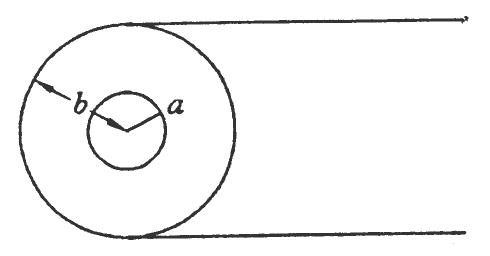
\includegraphics[height=3 cm]{images/q5_1.jpg}
        \caption{题\thequestion}
    \end{figure}
\end{question}

\begin{question}
    在电磁波传播问题中,试推出平面单色电磁波在两种介质交界面处的反射定律和折射定律。
\end{question}

\begin{question}
    写出单色电磁波在导体中的透入深度d。    
\end{question}